\chapter{Nuclear Fuel Depletion} \label{ch:burnupEquations}
Over the life time of a nuclear reactor the composition of the fuel changes from being exposed to a neutron rich environment. The changes in fuel composition have an important impact on the reactor power distribution, stability and control. Reactor efficiency as well as fuel utilization and economics are also greatly influenced from changes in fuel composition. As a nuclear reactor operates through time, the composition of the fuel elements changes due to fission, radioactive decay and neutron capture reactions. This change in composition is important because nuclear reaction rates are dependent on the material they occur. Fission rates are most important to calculate in order to maintain core critically. Not only does fissile material deplete producing fission products but fertile material can be converted into new fissile material. 

A complete depletion calculation would involve the simultaneous solution of the neutron transport equation along with the isotopic evolution of thousands of fission products and fissile material depletion. This is not possible in practice and approximations to these calculations must be done. The neutron transport and fuel depletion calculations are done separately and their coupling is often done with predictor corrector methods. During neutron transport calculations fuel composition is assumed to be constant. For depletion, reaction rates are assumed to be constant. This process is repeated until a stopping criteria is reached. 

In traditional light water reactors, fuel elements are housed in fuel rod bundles, which are not allowed to move during operation. Because molten salt reactors are liquid fueled, they can be refueled and have fission products processed online. In addition to online processing, fissial material circulates through the reactor loop. These unique design features of molten salt reactors produce new challenges for fuel depletion calculations. The following sections discuss the nuclear reactions involved in the production of radionuclides, neutron transport and the burnup equations.

\section{Nuclear Reactions}

\subsection{Radioactive Decay}
When the nucleus of an atomic element is unstable it can undergo spontaneous transformation into a different element by the emission of energy and or particles \cite{duderstadt1976}. The most relevant modes for decay in burnup calculations are $\alpha$ decay, proton emission, neutron emission, $\beta^{-}$ and $\beta^{+}$. A summary of these decay modes are shown in Table \ref{tab:decayModes} \cite{pusaThesis}. The rate at which a nuclide $i$ changes as a function of time is proportional to its decay constant $\lambda_{i}$ and the decay of other nuclides which contribute as a source to nuclide $i$  \cite{duderstadt1976}, 

\begin{equation}
    \frac{dn_{i}}{dt} = \sum_{j=1}^{N} \lambda_{j\rightarrow i}n_{j}(t) -\lambda_{i} n_{i}(t).
    \label{eq:decaySingleMode}
\end{equation}

\noindent The radioactive decay constant $\lambda$ is a natural constant and is related to the half life of the nuclide. This relation is,

\begin{equation}
    \lambda = \frac{\ln(2)}{T_{1/2}}.
\end{equation}

\noindent As the half life of the isotope decreases, its decay constant increases. 

Some nuclides have more than one mode of decay. Some of these decay modes compete with one another such as $\beta^{+}$ and electron capture. When nuclide \textit{i} has more than one decay mode, its decay constant is a summation of all $k$ decay modes,

\clearpage

\begin{table}[t]
    \caption{\label{tab:decayModes} Summary of Decay Modes where Z is atomic number and A is mass number \cite{pusaThesis}}
    \centering
    \begin{tabular}{c|c|c}
    \hline
    \textbf{Mode of decay} & \textbf{Daughter nuclide} & \textbf{By-product nuclide} \\ [0.5ex] 
    \hline
    \hline
    \\ [-1em]
    $\alpha$ decay & (Z - 2, A - 1) & ${}^{4}$He \\ \hline 
    \\ [-1em]
    Proton emission & (Z - 1, A - 1) & ${}^{1}$H \\ \hline
    \\ [-1em]
    Neutron emission & (Z, A - 1) & - \\ \hline
    \\ [-1em]
    $\beta^{-}$ & (Z + 1, A) & - \\ \hline
    \\ [-1em]
    $\beta^{+}$ & (Z - 1, A) & - \\ \hline
    \end{tabular}
\end{table}

\clearpage

\begin{equation}
    \lambda_{i} = \lambda_{i,1} + \lambda_{i,2} + \lambda_{i,3} ... = \sum_{k} \lambda_{i,k}.
\end{equation}

\noindent While total decay is sufficient for use in the loss of nuclide \textit{i} from Equation \ref{eq:decaySingleMode}, a branching ratio must be used to denoted the fraction of nuclide \textit{j} which decays into \textit{i}. The branching ratio is defined as,

\begin{equation}
    b_{j\rightarrow i} = \frac{\lambda_{j\rightarrow i}}{\lambda_{j}}.
\end{equation}

\noindent For nuclide \textit{j} which has multiple decay modes k, the branching ratio denotes the fraction of decays for nuclide \textit{j} which produce nuclide \textit{i}. Substituting this relation into Equation \ref{eq:decaySingleMode},

\begin{equation}
    \frac{dn_{i}}{dt} = \sum_{j=1}^{N} b_{j\rightarrow i}\lambda_{j}n_{j}(t) -\lambda_{i} n_{i}(t).
    \label{eq:decay}
\end{equation}




\subsection{Neutron Induced Reactions}
Neutron induced reactions follow the schematic shown in Figure \ref{fig:nuclearReaction}.  The projectile neutron encounters a target, resulting in the nuclear reaction. In this reaction, the neutron is denoted by \textit{a} and the target by \textit{b}, \textit{c} and \textit{d} are the resulting products. These reactions are often written in the following notation \cite{duderstadt1976},

\begin{equation*}
    b (a,c) d 
\end{equation*}



The frequency of a reaction is governed by the probability at which it can occur. This probability is related to the  cross section. The microscopic cross section is a factor that characterizes the probability of a neutron-nuclear reaction with an atomic nucleus \cite{duderstadt1976}. Specifically, the formal definition of the microscopic cross section is,

\begin{equation}
    \sigma = \frac{\text{Number of reactions} / \text{nucleus} / \text{sec}}{\text{Number of incident neutrons} / \text{cm}^{2} / \text{sec}} = \frac{(R/N_{i})}{\phi},
\end{equation}

\clearpage

\begin{figure}[b]
  \centering
  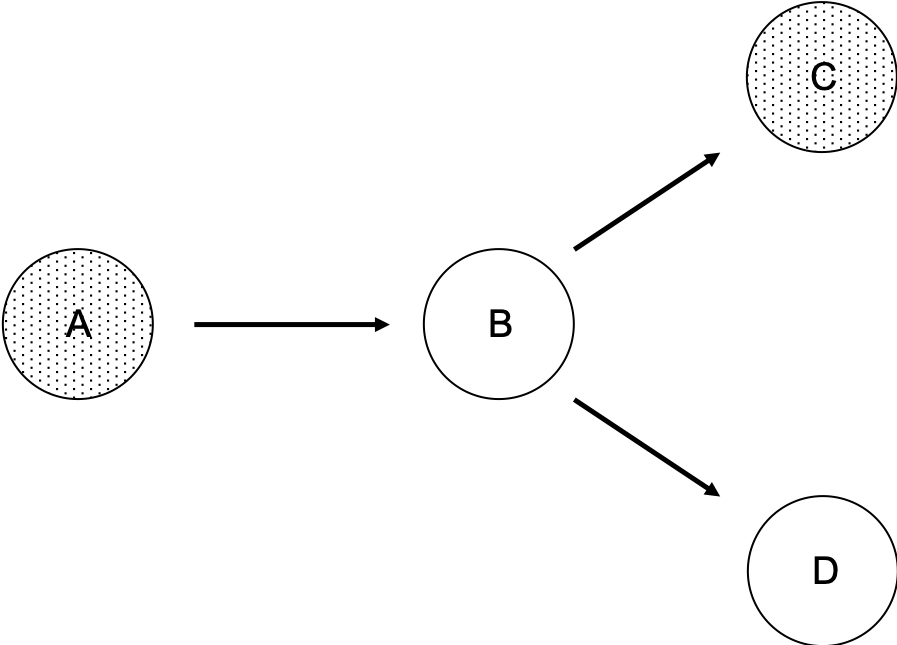
\includegraphics[width=3.0in]{images/chapter-2/nuclearReaction.png}\\
  \caption{Schematic of general nuclear reaction}
  \label{fig:nuclearReaction}
\end{figure} 

\clearpage

\begin{equation*}
    R = \bigg[\frac{\# \text{ of reactions}}{\text{cm}^{2}\cdot \text{sec}}\bigg], \quad \sigma = \big[\text{cm}^{2}\big], \quad \phi = \bigg[\frac{\# \text{ of neutrons}}{\text{cm}^{2}\cdot \text{sec}} \bigg], \quad n_{i} = \bigg[\frac{\# \text{ of atoms}}{\text{cm}^{3}}\bigg].
\end{equation*}

There are a number of neutron induced reactions that occur in a nuclear reactor. They can be divided into two main categories: scattering and absorption. Scattering reactions can then be further divided into elastic and inelastic reactions. Elastic scattering reactions, denoted by $(n,n)$ are those reactions in which an incoming neutron scatters off of a nucleus, changing the neutrons energy and direction. In some cases the neutron can be absorbed into the nucleus for a short time, before being ejected. This may leave the nucleus in an excited state before returning to its initial state. These type of reactions are noted by $(n,n')$ and are known as inelastic scattering. 

Absorption reactions are those in which a neutron is absorbed by the atomic nucleus. The resulting products from these reactions include, energy, neutrons, protons and $\alpha$ particles. A summary of these reactions which are relevant in burnup calculations are shown in Table \ref{tab:reactionModes} \cite{pusaThesis}. The change in a nuclides concentration as a function of time for a general absorption reaction is,

\begin{equation}
    \frac{dn_{i}}{dt} = \sum_{j=1}^{N} \sum_{k=1}^{K}\gamma_{j\rightarrow i,k}\sigma_{k,j}\phi n_{j}(t) - \phi\sum_{k=1}^{K} \sigma_{k,i}n_{i}(t),
    \label{eq:neutronIndecedReaction}
\end{equation}

\noindent where $\gamma_{j\rightarrow i,k}$ is the fraction of nuclide \textit{i} from nuclide \textit{j} through reaction \textit{k}. The first term in Equation  \ref{eq:neutronIndecedReaction} is the generation from the reaction of nuclide. First each nuclide is summed over, followed by a summation of each reaction for nuclide \textit{j}. If reaction \textit{k} results in generating nuclide \textit{i}, then $\sigma_{k,j}$ and $\gamma_{j\rightarrow i,k}$ are both nonzero. The second term in Equation \ref{eq:neutronIndecedReaction} is the loss of nuclide \textit{i} from reaction \textit{k}. For each nuclide \textit{i} a summation is taken over all possible neutron induced reactions. 


The microscopic cross section characterizes the probability that a neutron will have a reaction with a single nucleus. Often it is required to understand how neutrons will interact with macroscopic chunk of the material \cite{duderstadt1976}. The macroscopic cross section provides the 

\clearpage

\begin{table}[p]
    \caption{\label{tab:reactionModes} Summary of Decay Modes where Z is atomic number and A is mass number \cite{pusaThesis}}
    \centering
    \begin{tabular}{c|c|c}
    \hline
    \textbf{Mode of reaction} & \textbf{Daughter nuclide} & \textbf{By-product nuclide} \\ [0.5ex] 
    \hline
    \hline
    \\ [-1em]
    (n,2n) & (Z, A - 1) & - \\ \hline 
    \\ [-1em]
    (n,3n) & (Z, A - 2) & - \\ \hline 
    \\ [-1em]
    (n,4n) & (Z, A - 3) & - \\ \hline 
    \\ [-1em]
    (n,$\gamma$) & (Z, A + 1) & - \\ \hline 
    \\ [-1em]
    (n,p) & (Z - 1, A) & ${}^{1}H$ \\ \hline 
    \\ [-1em]
    (n,d) & (Z - 1, A - 1) & ${}^{2}$H \\ \hline 
    \\ [-1em]
    (n,t) & (Z - 1, A - 2) & ${}^{3}$H \\ \hline 
    \\ [-1em]
    (n,${}^{3}$He) & (Z - 2, A - 2) & ${}^{3}$He \\ \hline 
    \\ [-1em]
    (n,$\alpha$) & (Z - 2, A - 3) & ${}^{4}$He \\ \hline 
    \\ [-1em]
    Fission & fission products & - \\ \hline
    \end{tabular}
\end{table}

\clearpage

\noindent ability to compute how a large portion of material will react under a flux of particles or energy. This macroscopic cross section is the computation of the atomic number density multiplied by the microscopic cross section. For a material consisting of multiple atomic elements, the macroscopic cross section of reaction $x$ is computed by,

\begin{equation}
    \Sigma_{x} = \sum_{i=1}^{N}n_{i}\sigma_{i,x},
\end{equation}

\noindent The macroscopic cross section can be thought of as the probability per length path that a neutron will have a reaction with the nucleus \cite{duderstadt1976}. 

When fissile material undergoes a neutron absorption (to relate it to the previous paragraphs), neutron induced fission can occur releasing neutrons, energy and fission products. Typically, fission is a two-body reaction, meaning that the target nucleus splits into two isotopes of smaller atomic number. The independent fission product yield is the expected fraction a nuclide is produced for a single fission event. Because the cross section is dependent on the incident neutron energy, fission product yields dependent on the neutron energy. The yields of fission products for ${}^{235}$U for fast and thermal neutrons is shown in Figure \ref{fig:fissionYield}.



\section{Neutron Transport Equation}
The neutron transport equation describes the angular neutron density as a function of time, space and energy. Let the spatial position be denoted by $r$ and the energy of a neutron $E$. A neutron will travel in direction $\Omega$ and will scatter at angle $\Omega'$ and energy $E'$.  The neutron transport equation is,

\begin{equation}
    \frac{1}{v}\frac{\partial \varphi}{\partial t} + \Omega \cdot \nabla \varphi + \Sigma_{t}\varphi = \int_{4\pi} d\Omega'\int_{0}^{\infty}dE'\Sigma_{s}\varphi' + \frac{\chi}{4\pi}\int_{0}^{\infty}dE'\nu\Sigma_{f}\varphi,
    \label{eq:angularNeutronTransport}
\end{equation}

\noindent where 

\clearpage

\begin{figure}[t]
  \centering
  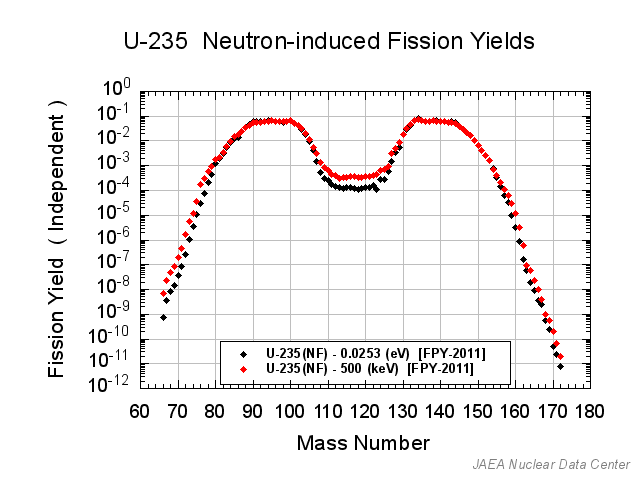
\includegraphics[width=5.5in]{images/chapter-2/fissionYield.png}\\
  \caption{Fission product yield for thermal and fast neutrons}
  \label{fig:fissionYield}
\end{figure} 

\clearpage

$\begin{aligned}
&\varphi = \varphi(r, E, \Omega) \equiv   \text{Angular neutron flux at energy } E \text{ and angle } \Omega  \\
&\varphi' = \varphi(r, E', \Omega') \equiv   \text{Angular neutron flux at energy } E' \text{ and angle } \Omega'  \\
& v = v(E) \equiv \text{ Neutron velocity} \\
&\Sigma_{t} = \Sigma_{t}(r, E) \equiv \text{ Total neutron cross section} \\
&\Sigma_{s} = \Sigma_{s}(E' \rightarrow E,\Omega' \rightarrow \Omega) \equiv \text{ Neutron scattering cross section from energy } E \\
& \text{ and angle } \Omega \text{ to energy } E' \text{ and angle } \Omega' \\
&\chi = \chi(E) \equiv \text{ Energy distribution of fission neutrons} \\
&\nu = \nu(E') \equiv \text{ Average number of neutrons released during fission at energy } E' \\ 
&\Sigma_{f} = \Sigma_{f}(E') \equiv \text{ Cross section for neutron fission at energy } E' 
\end{aligned}$

\vspace{0.5cm}

\noindent Starting from the left hand side of Equation \ref{eq:angularNeutronTransport} we have the change in neutron density with time, neutron streaming and neutron removal from reaction. On the right hand side is the source from a neutron scattering in from and different energy and angle, followed by the source from nuclear fission. The source for the scattering term must be integrated over all angles and energy and the same for the fission source. The angular neutron flux cannot be directly used in the neutron induced reaction equations presented before. These equations require the scalar flux, which is the integral over all angles for the angular neutron flux,

\begin{equation}
    \phi(r,E) = \int \varphi(r,E,\Omega)d \Omega.
\end{equation}

Angular dependence for the scattering source can be handled through the use of Legendre expansions or spherical harmonics. Spacial angular dependence is often treated with Gauss-Legendre quadratures such as the Sn or Pn equations, such methods are out of the scope of this work \cite{millerCompTransport}. The energy dependence in Equation \ref{eq:angularNeutronTransport} is almost always handled using the multigroup approximation. This approximation works by dividing up the energy dependence in groups by applying an energy interval for each group and integrating over that interval. The group cross sections are defined in a way to conserve the reaction rates. The multigroup constants are defined by \cite{millerCompTransport} \cite{duderstadt1976},

\begin{equation}
    \Sigma_{s}^{gg'} = \frac{\int_{g}^{g-1}\int_{g'}^{g'-1}\Sigma_{s}(r,E'\rightarrow E,t)\varphi(r,E',t) dE'dE}{\int_{g}^{g-1}\varphi(r,E,t) dE},
\end{equation}

\begin{equation}
    \Sigma_{t}^{g} = \frac{\int_{g}^{g-1}\Sigma_{t}(r,E,t)\varphi(r,E,t) dE}{\int_{g}^{g-1}\varphi(r,E,t) dE},
\end{equation}

\begin{equation}
    \nu\Sigma_{f}^{g} = \frac{\int_{g}^{g-1}\nu\Sigma_{f}(r,E,t)\varphi(r,E,t) dE}{\int_{g}^{g-1}\varphi(r,E,t) dE},
\end{equation}

\begin{equation}
    \chi^{g} = \int_{g}^{g-1}\chi(E) dE,
\end{equation}

\begin{equation}
    \varphi^{g} = \int_{g}^{g-1}\varphi(r,E,t) dE.
\end{equation}

The time variance in Equation \ref{eq:angularNeutronTransport} is most often neglected for reactor analysis. Instead the problem is transformed into an eigenvalue problem. Although there are multiple different eigenvalue formulations, the $\lambda$ (k-effective, criticality) eigenvalue is the most common \cite{millerCompTransport}. If Equation \ref{eq:angularNeutronTransport} is written in matrix vector form, then the criticality equation is,

\begin{equation}
    \boldsymbol{A}\boldsymbol{\varphi} = \frac{1}{\lambda}\boldsymbol{B}\boldsymbol{\varphi}.
\end{equation}

\noindent where $\lambda$ is the largest of the eigenvalues and can be found using the power iteration. When $\lambda$ is greater than 1 then the reactor is supercritical and the neutron population will increase over time. If $\lambda$ is less than 1 the system is subcritical and the neutron population will decrease over time. If $\lambda$ is equal to 1 then the system is critical and the neutron population will remain constant \cite{duderstadt1976}. 


\section{Burnup Equations}
Nuclear burnup calculations solve a set of first order ODE's which aim to simulate the isotopic concentrations of radionuclides in a nuclear reactor. These equations are important in reactor calculations because the neutronic properties and neutron distributions in the reactor is dependent on composition of the environments material. After a neutron transport solve, the cross sections and scalar neutron flux are collapsed into a single energy group. Because of the manner in which the groups are collapsed, the reaction rates from the multigroup equations equal the reaction rates for the single group. Over a single burn up calculation step all cross sections and the scalar neutron flux is assumed to be constant. When solving the depletion equations, the reactor is often subdivided into finite volume depletion zones. Each depletion zone with have different material, and differing neutron flux, this results in the reaction rates varying between each region. Using volume average operators and the multigroup approximation, the neutron flux and microscopic cross section is collapsed into single values for each depletion zone \cite{aarnoThesis},

\begin{equation}
    \overline{\sigma}_{k,j} = \frac{\int_{V}\int_{0}^{\infty}\sigma_{k,j}(r,E)\phi(r,E) dEdV}{\int_{V}\int_{0}^{\infty}\phi(r,E) dEdV},
\end{equation}

\begin{equation}
    \overline{\phi} = \frac{1}{V}\int_{V}\int_{0}^{\infty}\phi(r,E)dEdV.
\end{equation}

\begin{equation}
    \overline{n}(t) = \frac{1}{V}\int_{V}n(r,t)dV
\end{equation}

\noindent This results in the set of ODE's of the form,

\begin{equation}
    \frac{d\overline{n}_{i}}{dt} = \sum_{j=1}^{N}\bigg(b_{j\rightarrow i}\lambda_{j} + 
    \sum_{k=1}^{K}\gamma_{j\rightarrow i,k}\overline{\sigma}_{k,j}\overline{\phi} \bigg)\overline{n}_{j}(t) - \bigg(\lambda_{i} + \overline{\phi}\sum_{k=1}^{K} \overline{\sigma}_{k,i}\bigg)\overline{n}_{i}(t).
    \label{eq:LWRDepletion}
\end{equation}

There are multiple methods for solving the isotopic concentrations in nuclear reactors \cite{isotalo2011} \cite{pusa2010} \cite{akio2007}. Normal numerical integration techniques such as Runge Kutta face complications because of the various orders of magnitude for the decay constants of short and long lived nuclides. This results in a stiff system of ODE's, which are difficulty and costly to solve. Recently, matrix exponential methods have become popular for depletion calculations because of their high level of accuracy \cite{pusaThesis} \cite{aarnoThesis}. 

\subsection{Extension to Molten Salt Reactors}
Traditional nuclear reactors contain their fuel in a solid form that is unable to move during operation. These fuel elements are housed in pellets which are loaded in fuel rods. These rods are collected into fuel bundles which are then loaded into the reactor core for operation. Loading the reactor core with fuel in this form does not allow the material to transport through the reactor loop. Molten salt reactors work with a liquid form of the fuel that is dissolved in a molten salt. This liquid form of the fuel allows it to transport through the reactor loop during operation. Thus the depletion equations used in traditional reactors no longer hold true for molten salt reactors. Equation \ref{eq:LWRDepletion} must be modified to include the change in nuclide concentration with fluid movement: convection and diffusion. 

Depletion calculations in MSRs can be better represented by the multicomponent chemical species transport equation. The species transport equation is derived by a conservation of mass basis which accounts for change in time, convective and diffusion transport and rate of generation from reaction \cite{bird2006}. Equation \ref{eq:speciesTransportEquation} is the species transport equation for species \textit{i}. 

\begin{equation}
    \underbrace{\frac{\partial \rho_{i}}{\partial t}}_{\substack{\text{Change in} \\
    \text{density} \\
    \text{with time}}} + 
    \underbrace{\nabla \cdot \rho_{i}(r,t)\boldsymbol{v}}_{\substack{\text{Transport} \\
    \text{with fluid} \\
    \text{velocity}}}
    + \underbrace{\nabla \cdot j_{i}(r,t)}_{\substack{\text{Transport} \\
    \text{with mass} \\
    \text{diffusion}}} = 
    \underbrace{R_{i}(r,t)}_{\substack{\text{Generation} \\
    \text{from} \\
    \text{reaction}}}
    \label{eq:speciesTransportEquation}
\end{equation}

\noindent It is important to note that the velocity in the second term must be the averaged velocity for the concentration of interest. In Equation \ref{eq:speciesTransportEquation} for example, the concentration units are for mass concentration or density. This means that the velocity used in the second term must be the mass averaged velocity \cite{zackThesis}. 

Equation \ref{eq:LWRDepletion} is simply the rate of generation for nuclide species $\textit{i}$ and can be plugged in for $r_{i}$ in Equation \ref{eq:speciesTransportEquation}. Before it can be plugged in, the units in Equation \ref{eq:LWRDepletion} need to be transformed from atoms per volume to mass per volume using Avogadros constant the molar mass, $n_{i} = \rho_{i}N_{A} / M_{i}$. Using this relation and plugging in Equation \ref{eq:LWRDepletion} into \ref{eq:speciesTransportEquation} results in the MSR depletion equation,


\begin{equation}
\begin{split}
    \frac{\partial \rho_{i}}{\partial t}
    + \nabla \cdot \rho_{i}(r,t)\boldsymbol{v}
    + \nabla \cdot j_{i}(r)
    &=
    \sum_{j=1}^{N}\frac{M_{i}}{M_{j}}\bigg(b_{j\rightarrow i}\lambda_{j} + 
    \sum_{k=1}^{K}\gamma_{j\rightarrow i,k}\sigma_{k,j}(r)\phi(r,t) \bigg)\rho_{j}(r,t)\\
    &- \bigg(\lambda_{i} + \phi(r,t)\sum_{k=1}^{K} \sigma_{k,i}(r)\bigg)\rho_{i}(r,t).
\end{split}
    \label{eq:MSRDepletion}
\end{equation}

The MSR depletion equation represents the change in an isotopes density via fluid transport, mass diffusion and nuclear reactions. Equation \ref{eq:MSRDepletion} is a nonlinear PDE, first order in time and second order in space. It should be noted that Equation \ref{eq:LWRDepletion} was already discretized in space. For completeness $\sigma_{k,j}$ and $\phi$ are also functions of space and time in Equation \ref{eq:MSRDepletion} however, the scalar flux is for a single energy group. Solving Equation \ref{eq:MSRDepletion} is the primary topic and will be discussed through out the remainder of the dissertation.

\subsection{Mass Transport Models}
Fission products that are generated in MSRs are often categorized based on their phase and chemical behavior in the molten salt. The common categories are \cite{grimes1975}: 

\begin{enumerate}
    \item Salt seekers
    \item Noble metals
    \item Noble gases
\end{enumerate}

\noindent Salt seekers are fission products which form halide compounds which are soluble in the molten salt. Noble metals, are elements which under go redox reactions and are reduced to their neutral state. These fission products form metallic compounds which tend to collect on liquid-solid or liquid-gas interfaces. When collecting on liquid-solid surfaces within the flow loop, these fission products can plate a metallic film on the surface which can possibly work to reduce corrosion. Noble metals can also decay which doses the surface with radiation and decay heat. Noble gases such as Xe and Kr are gases which form in the liquid salt from nuclear reactions. These elements can be dissolved in the liquid salt or extracted via gas stripping. In addition, these products may nucleate and/or become trapped in reactor equipment such as a graphite moderator. 

A first order rate model is utilized in modeling mass transfer from liquid to solid and liquid to gas surfaces. At the interface, the flux normal to the surface is defined as \cite{bird2006}:

\begin{equation}
    j = k_{\text{loc}} \Delta \rho,
    \label{eq:interface_bc_mass_transfer}
\end{equation}

\noindent where $j$ is the mass flux [kg/s/m$^{2}$] and $k_{i, \text{loc}}$ is the local mass transfer coefficient [m/s] in terms of density. Depending of the direction of mass transfer the sign of $j_{i}$ can be positive or negative based on the concentration gradient of $\Delta \rho_{i}$. On of the key features of using this previous relation is understanding and calculating the mass transfer coefficient $k$ in its appropriate form. This coefficient will depend upon the fluid profile and geometry within the local region of mass transfer. There are many analytic and empirical relations that can be used to calculate $k$ for different situations. An exhausted summary of these calculation methods can be found in Perry's Chemical Engineers' Handbook \cite{perry2007}.

Equations of the form Eq. \ref{eq:interface_bc_mass_transfer} are sufficient for approximating the mass transfer of a liquid to a solid surface and was utilized in modeling noble metal wall deposition during the molten salt reactor experiment (MSRE) \cite{kedl1972}. For this case, noble metals are transported from the liquid phase to the sold surfaces within the reactor loop. This model is call wall deposition and is represented as:

\begin{equation}
    j = k(\rho_{\text{bulk}} - \rho_{\text{surface}}).
\end{equation}

Liquid gas transport is a bit more involved than the wall deposition model. For a liquid-gas system, the species fluxes across the interface as represented by the equation below:

 \begin{equation}
	j = k_{G}(\rho^{g}_{\text{bulk}} - \rho^{g}_{i}) = k_{L}(\rho^{l}_{i} - \rho^{l}_{\text{bulk}})
	\label{eq:convection_boundary_condition},
\end{equation}

\noindent where $k_{G}$ is the gas-phase mass transfer coefficient, $k_{L}$ is the liquid-phase mass transfer coefficient, $\rho^{g}_{bulk}$ is the bulk concentration in the gas phase, $\rho^{l}_{bulk}$ is the bulk concentration in the liquid phase, $\rho^{g}_{i}$ is the concentration at the interface on the gas side, and $\rho^{l}_{i}$ is the concentration at the interface on the liquid side. Because the concentration at the interface of a liquid-gas system is difficult to establish, it is convenient to rewrite Eq. (\ref{eq:convection_boundary_condition}) as:

 \begin{equation}
	j = K_{G}(\rho^{g}_{\text{bulk}} - \rho^{g}_{*}) = K_{L}(\rho^{l}_{*} - \rho^{l}_{\text{bulk}})
	\label{eq:overall_convection_boundary_condition},
\end{equation}

\noindent where $k_{G}$ and $k_{L}$ have been replaced by $K_{G}$ and $K_{L}$, the overall mass transfer coefficients, $\rho^{g}_{*}$ is the gas composition in equilibrium with the liquid, and $\rho^{l}_{*}$ is the liquid composition in equilibrium with the gas. For liquid-gas systems, these equilibrium concentrations can be calculated using Henry's law. 

When the gas has a low solubility in the liquid, the process is dominated by the liquid side resistance \cite{bird2006}. Both Xe and Kr were found to be only slightly soluble in salt during the MSRE \cite{kedl1972}. Because of this, the mass transfer flux becomes:

\begin{equation}
    j = k_{l}(\rho^{l}_{*} - \rho^{l}_{\text{bulk}}).
\end{equation}

\subsection{Boundary Conditions}
Mathematically, there are three types of boundary conditions for Equation \ref{eq:MSRDepletion}: Dirichlet, Neumann and Robin. Each of these boundary conditions are implemented in a way that permit inlet and outlet flow. Dirichlet boundary conditions specify a single constant value at the boundary. A Neumann boundary condition specifies the gradient normal to the boundary surface to be constant. The Robin boundary condition includes both the dependent variable and gradient are included. Table \ref{tab:boundaryConditions} summarizes each of the boundary conditions.

\begin{table}[h]
    \caption{\label{tab:boundaryConditions} Boundary Conditions}
    \centering
    \begin{tabular}{c|c}
    \hline
    \textbf{Boundary condition} & \textbf{Form} \\ [0.5ex] 
    \hline
    \hline
    \\ [-0.75em]
    Dirichlet & $\rho_{i}(x_{b}) = C$\\ [0.8ex] \hline \\ [-0.75em]
    Neumann & $\frac{\partial \rho_{i}}{\partial x}(x_{b}) = C$\\ [0.8ex] \hline \\ [-0.75em]
    Robin & $a\rho_{i}(x_{b}) + b\frac{\partial \rho_{i}}{\partial x}(x_{b}) = C$\\ [0.8ex] \hline
    \end{tabular}
\end{table}



